\documentclass[a4paper,12pt]{article}
%%%%%%%%%%%%%%%%%%%%%%%%%%%%%%%%%%%%%%%%%%%%%%%%%%%%%%%%%%%%%%%%%%%%%%%%%%%%%%%%%%%%%%%%%%%%%%%%%%%%%%%%%%%%%%%%%%%%%%%%%%%%%%%%%%%%%%%%%%%%%%%%%%%%%%%%%%%%%%%%%%%%%%%%%%%%%%%%%%%%%%%%%%%%%%%%%%%%%%%%%%%%%%%%%%%%%%%%%%%%%%%%%%%%%%%%%%%%%%%%%%%%%%%%%%%%
\usepackage{eurosym}
\usepackage{vmargin}
\usepackage{amsmath}
\usepackage{graphics}
\usepackage{epsfig}
\usepackage{subfigure}
\usepackage{fancyhdr}
%\usepackage{listings}
\usepackage{framed}
\usepackage{graphicx}
\usepackage{amsmath}
\usepackage{chngpage}
%\usepackage{bigints}


\setcounter{MaxMatrixCols}{10}
%TCIDATA{OutputFilter=LATEX.DLL}
%TCIDATA{Version=5.00.0.2570}
%TCIDATA{<META NAME="SaveForMode" CONTENT="1">}
%TCIDATA{LastRevised=Wednesday, February 23, 2011 13:24:34}
%TCIDATA{<META NAME="GraphicsSave" CONTENT="32">}
%TCIDATA{Language=American English}

%\pagestyle{fancy}
%\setmarginsrb{20mm}{0mm}{20mm}{25mm}{12mm}{11mm}{0mm}{11mm}
%\lhead{MA4413} \rhead{Mr. Kevin O'Brien}
%\chead{Statistics For Computing}
%\input{tcilatex}

\begin{document}
\begin{center}
       
\includegraphics[scale=0.55]{shieldtransparent2}
\end{center}

\begin{center}
\vspace{1cm}
\large \bf {FACULTY OF SCIENCE AND ENGINEERING} \\[0.5cm]
\normalsize DEPARTMENT OF MATHEMATICS AND STATISTICS \\[1.25cm]
\large \bf {REPEAT EXAMINATION PAPER 2013} \\[1.5cm]
\end{center}

\begin{tabular}{ll}
MODULE CODE: MA4605 & SEMESTER: Summer 2013 \\[1cm]
MODULE TITLE: Chemometrics & DURATION OF EXAM: 2.5 hours \\[1cm]
LECTURER: Mr. Kevin O'Brien & GRADING SCHEME: 80 marks \\
& \phantom{GRADING SCHEME:} \footnotesize {70\% of module grade} \\[0.8cm]
\\[1cm]
\end{tabular}
\begin{center}
{\bf INSTRUCTIONS TO CANDIDATES}
\end{center}

{\noindent \\ Scientific calculators approved by the University of Limerick can be used. \\
Formula sheet and statistical tables provided at the end of the exam paper.\\
Students must attempt any 4 questions from 5.}
\newpage



% - Section 1 Inference Procedures
        % a. Parametric
        % b. Non Parametric
% - Section 2 Linear Models
        % a. SLR
        % b. MLR
% - Section 3 Linear Models
        % a. Robust Regression
        % b. AIC
% - Section 4 Statistical Process control
        % a. Control Limits
        % b. Theory Questions
        % c. Interpreting Charts
        % d. CUSUM and ARL
% - Section 5 Experimental Design 1
        % a. Definitions for ED
        % b. One Way ANOVA
% - Section 6 Experimental Design 2
        % a.
        % b.


\subsection*{Question 1. (20 marks) Inference Procedures}
\begin{itemize}
\item The nicotine content in blood can be determined by gas chromatography down to concentrations of 1 ng/ml. The concentration of nicotine was determined in each of two samples of known concentrations 10 ng/ml and 50 ng/ml.
\begin{framed}
\begin{verbatim}
Data: Sample (Lo): m = 10 ng/ml, n=14.

 8.40, 9.59, 9.38, 9.10, 10.78, 11.41, 9.94, 
10.08, 12.11, 9.10, 9.59, 10.36, 10.41, 10.52.

Data: Sample (Hi): m = 50 ng/ml, n=10.

47.5, 48.4, 48.8, 48.4, 46.8, 
46.2, 48.6, 50.6, 45.5, 46.1.
\end{verbatim}
\end{framed}
A research team evaluated both samples to determine whether or not the samples were similar in terms of measures of centrality and dispersion, before the trial commenced.  \\  \\ The following blocks of \texttt{R} code (i.e blocks 1 to 6) are based on the data for this assessment. \\ 
\begin{itemize}
\item[(a)] (10 Marks) Each of the six blocks of code describes a statistical inference procedure. Provide a brief description for each procedure.
\item[(b)] (10 Marks) Write a short report on your conclusion for this assessment, clearly indicating which blocks of \texttt{R} code you felt were most relevant, and explain why. 
\end{itemize}

\begin{itemize}
\item[\textbf{Block 1}]
\begin{framed}
\begin{verbatim}

        F test to compare two variances

data:  Lo and Hi
F = 0.3945, num df = 13, denom df = 9, p-value = 0.1246
alternative hypothesis: 
 true ratio of variances is not equal to 1
95 percent confidence interval:
 0.1029905 1.3066461
sample estimates:
ratio of variances 
         0.3945149
\end{verbatim}
\end{framed}

\item[\textbf{Block 2}]
\begin{framed}
\begin{verbatim}
> shapiro.test(Lo)

        Shapiro-Wilk normality test

data:  Lo
W = 0.9779, p-value = 0.9609
> shapiro.test(Hi)

        Shapiro-Wilk normality test

data:  Hi
W = 0.9496, p-value = 0.6634
\end{verbatim}
\end{framed}
\bigskip
\item[\textbf{Block 3}]
\begin{framed}
\begin{verbatim}
> t.test(Lo,Hi)

        Welch Two Sample t-test

data:  Lo and Hi
t = -67.374, df = 14.016, p-value < 2.2e-16
alternative hypothesis: 
   true difference in means is not equal to 0
95 percent confidence interval:
 -38.83294 -36.43706
sample estimates:
mean of x mean of y 
   10.055    47.690 
\end{verbatim}
\end{framed}
\newpage
\item[\textbf{Block 4}]
\begin{framed}
\begin{verbatim}
> t.test(Lo,Hi,var.equal=TRUE)

        Two Sample t-test

data:  Lo and Hi
t = -72.6977, df = 22, p-value < 2.2e-16
alternative hypothesis: 
   true difference in means is not equal to 0
95 percent confidence interval:
 -38.70863 -36.56137
sample estimates:
mean of x mean of y 
   10.055    47.690 

\end{verbatim}
\end{framed}



\item[\textbf{Block 5}]
\begin{framed}
\begin{verbatim}
> ks.test(Lo,Hi)

        Two-sample Kolmogorov-Smirnov test

data:  Lo and Hi
D = 1, p-value = 1.02e-06
alternative hypothesis: two-sided

\end{verbatim}
\end{framed}
%------------------------------------------------------------------%
\item[\textbf{Block 6}]
\begin{framed}
\begin{verbatim}
 wilcox.test(Lo,Hi)

        Wilcoxon rank sum test


data:  Lo and Hi
W = 0, p-value = 1.02e-06
alternative hypothesis: 
	true location shift is not equal to 0

\end{verbatim}
\end{framed}
\end{itemize}

\end{itemize} % End of Question Block
%--------------------------------------------------------------------------------------------------------%
%--------------------------------------------------------------------------------------------------------%
\newpage
%Q2A Simple Linear Linear Regression
%Q2B Method Comparison Studies

\subsection*{Question 2. (20 marks) Linear Models }
%--------------------------------------------------------------------------------------------------------%
\begin{itemize} %Start of Question


%-------------------------------Start of Question 2A%

\item[(a)]
The fluorescence of each of a series of acidic solutions of quinine with concentrations 0,10,20,30,40,50
was determined five times. The mean values and standard deviations of these determinations have
been obtained as follows:
\begin{center}
\begin{tabular}{|c|cccccc|}
         \hline
         % after \\: \hline or \cline{col1-col2} \cline{col3-col4} ...
         Means: & 4.0 & 21.2& 44.6& 61.8& 78.0 &105.2\\
        Std Deviations: &0.71& 0.84 &0.89 &1.64 &2.24 &3.03\\
         \hline
\end{tabular}
\end{center}
Two models have been fitted to the data. These models are described by the following \texttt{R} code output.


\begin{itemize}
\begin{framed}
\item[\textbf{Model 1}]
\begin{verbatim}
lm(formula = Means ~ Conc)

Coefficients:
Estimate Std. Error t value Pr(>|t|)
(Intercept) 2.9238 2.1648 1.351 0.248
Conc 1.9817 0.0715 27.715 1.01e-05 ***
---
Residual standard error: 2.991 on 4 degrees of freedom
Multiple R-squared: 0.9948,Adjusted R-squared: 0.9935
F-statistic: 768.1 on 1 and 4 DF, p-value: 1.008e-05
\end{verbatim}
\end{framed}
\begin{framed}
\item[\textbf{Model 2}]
\begin{verbatim}
weights=SdInt^(-2)/mean(SdInt^(-2))

lm(formula = Means ~ Conc, weights = weights)
Coefficients:
Estimate Std. Error t value Pr(>|t|)
(Intercept) 3.48066 1.15736 3.007 0.0397 *
Conc 1.96315 0.06765 29.018 8.4e-06 ***
---
Residual standard error: 2.034 on 4 degrees of freedom
Multiple R-squared: 0.9953,Adjusted R-squared: 0.9941
F-statistic: 842 on 1 and 4 DF, p-value: 8.396e-06
\end{verbatim}
\end{framed}
\end{itemize}
\begin{itemize}
%\item[i.] (2 marks) What is the regression equation for this fitted model?
%\item[ii.] (4 marks) Comment on the significance of the regression estimates.
\item[i.] (4 Marks) What kind of analyses have been performed in each of model 1 and model 2? Write down the linear model regression equation fitted by each of the two analyses.

\item[ii.] (3 Marks) Describe differences between the two models, making reference to the scatter-plot of the data on the next page. (Also present on the scatter-plot is a regression line fitted using the first analysis).
\item[iii.] (2 Marks) Based on the \texttt{R} code output, which model is the better fit?
%\item[iv.] (2 Marks) What is the Akaike information criterion? Descibe how it could be used in this context.
\end{itemize}
\newpage
\begin{center}
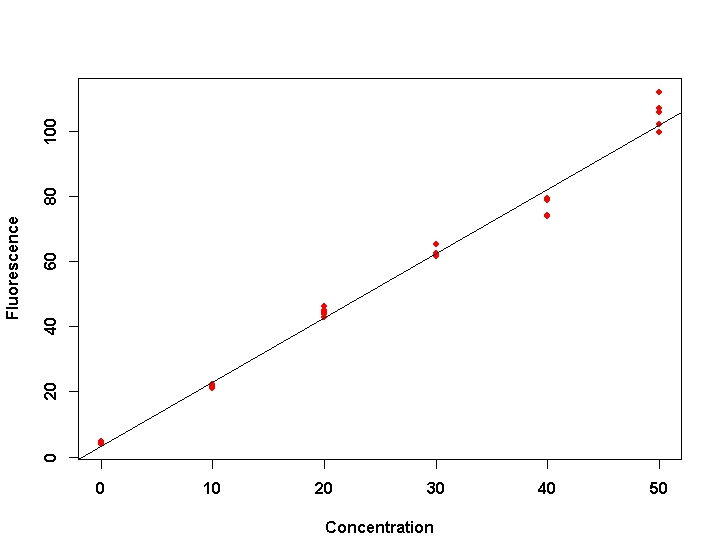
\includegraphics[scale=0.45]{ExamQ2plot2}
\end{center}.
%\begin{center}
%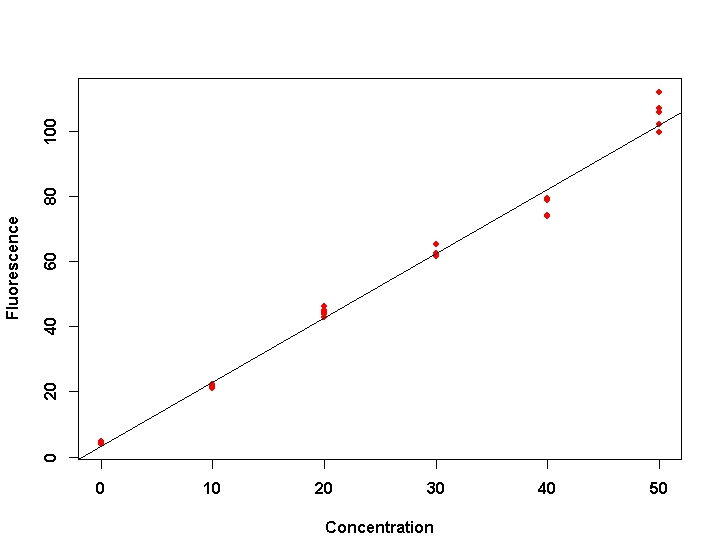
\includegraphics[scale=0.60]{ExamQ2plot2}
%\end{center}

%-------------------------------End  of Question 2A%
%-------------------------------Start of Question 2B%
%\item[(b)](6 marks)
%The scatter-plot contains the regression line for the fitted model. Three diagnostic plots, used to assess the suitability of the fitted model, are presented on the following pages. Provide a brief interpretation for each of the three diagnostic plots described in part(a). The scatter-plot for the data is also presented.

%\begin{center}
%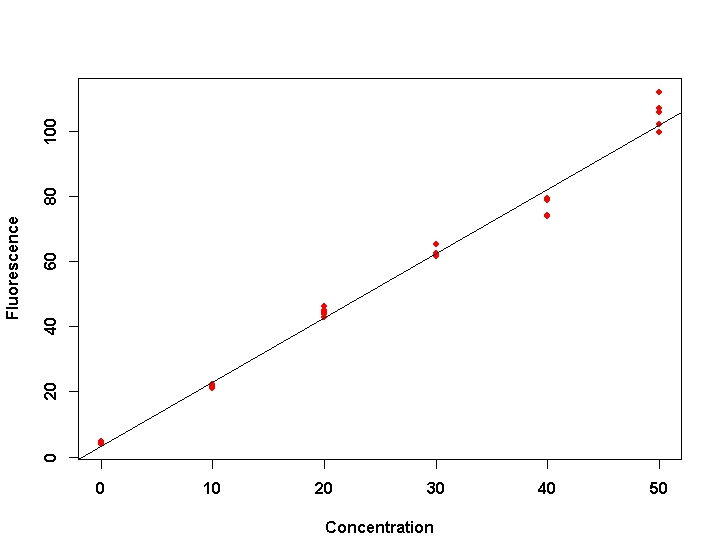
\includegraphics[scale=0.60]{ExamQ2plot2}
%\end{center}
%\newpage
%\begin{center}
%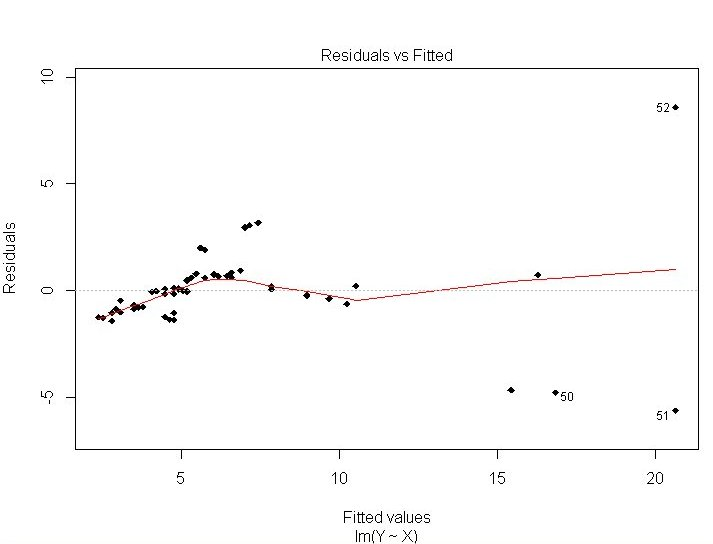
\includegraphics[scale=0.55]{ExamQ2diag1}
%\end{center}
%
%\begin{center}
%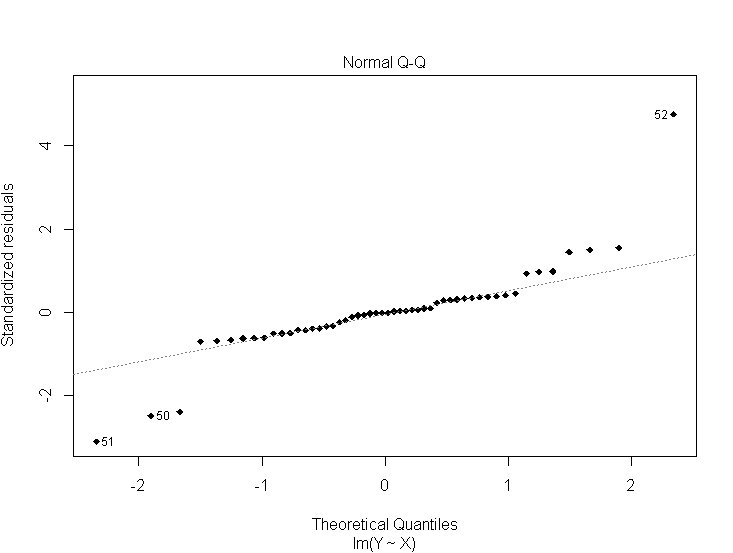
\includegraphics[scale=0.55]{ExamQ2diag2}
%\end{center}
%
%\begin{center}
%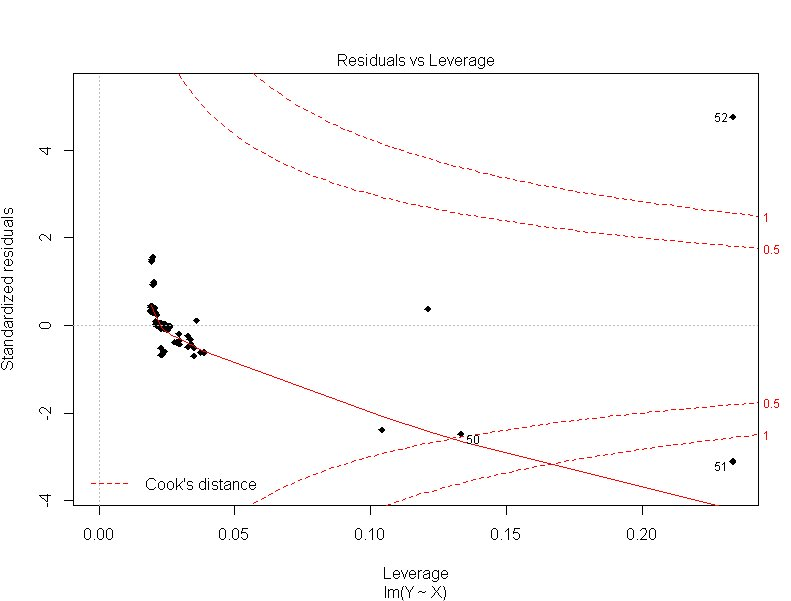
\includegraphics[scale=0.55]{ExamQ2diag3}
%\end{center}

%-------------------------------End  of Question 2B%

%-------------------------------Start of Question 2C%
\item[(b)] An ion-selective electrode (ISE) determination of sulphide from sulphate-reducing bacteria was compared with a gravimetric determination. Each pair of determinations were taken from the same sample. \\ \\The results obtained by both methods are expressed in milligrams of sulphide, and are tabulated below.
\begin{center}
\begin{tabular}{|c|cccccccccc|}
  \hline
  % after \\: \hline or \cline{col1-col2} \cline{col3-col4} ...
ISE method & 108 & 12& 152 & 3 & 106 & 11 &  128 & 12& 160& 128 \\
gravimetry & 105 & 16& 113 & 1 & 108 &  11 & 141 & 161 & 182& 118\\
  \hline
\end{tabular}
\end{center}
Two simple linear models are fitted to the data. Model C uses the gravimetric determination as an independent variable used to predict the ISE determination. Conversely, Model D uses the ISE determination as an independent variable used to predict the gravimetric determination. The relevant \texttt{R} output is presented on the following page.
%Method Comparison Studies
\newpage
\begin{itemize}
\begin{framed}
\item[\textbf{Model C}]
\begin{verbatim}
Call:
lm(formula = ISE ~ grav)
...
Coefficients:
            Estimate Std. Error t value Pr(>|t|)
(Intercept)  15.1125    28.8487   0.524    0.615
grav          0.6997     0.2543   2.751    0.025 *
....
\end{verbatim}
\end{framed}
\begin{framed}
\item[\textbf{Model D}]
\begin{verbatim}
Call:
lm(formula = grav ~ ISE)
..
Coefficients:
            Estimate Std. Error t value Pr(>|t|)
(Intercept)  38.6215    25.8542   1.494    0.174
ISE           0.6949     0.2526   2.751    0.025 *
....
\end{verbatim}
\end{framed}
\end{itemize}

\begin{itemize}
%\item[i.] (4 marks) Write the regression equation for both of the fitted models.
\item[i.] (3 marks) Is a simple linear regression model an suitable approach for this type of analysis? Explain why or why not? What alternative type of regression analysis might you recommend?
\item[ii.] (2 marks) Provide a brief description of the Bland-Altman plot. Discuss any shortcomings with this approach to method comparison.
\end{itemize}


%-------------------------------End  of Question 2B%






\newpage






%\item[(b)]
%Explain the following terms in the context of linear regression models.
%\begin{itemize}
%\item[i.] (2 marks) Influence,
%\item[ii.] (2 marks) Leverage,
%\item[iii.] (2 marks) Cook's Distance.	
%\end{itemize}

%---------------------%



%\item[(c)] (6 marks)
% Write a brief explanation of how robust regression differs from linear models computed using the \emph{Ordinary Least Squares method}, making reference to one particular weighting method only. Provide a description on how this weighting method works.









%%-------------------------------------%
%\subsection*{Question 3. (20 marks) Multiple Linear Regression Models }
%\begin{itemize}
%
%\item[(a)] Explain the following terms:
%\begin{itemize}
%\item[i.] (2 marks) Over-fitting,
%\item[ii.] (2 marks) Multicollinearity,
%\item[iii.] (2 Marks) Heteroscedascity.
%\end{itemize}
%\item[(b)] Answer the following questions related to model selection techniques for linear models.
%\begin{itemize}
%\item[i.] (2 marks) Explain why the adjusted $R^2$ value may differ in value from the corresponding multiple $R^2$ value for the same fitted model.
%\item[ii.] (2 marks) Explain how the \emph{Akaike information criterion} would used to compare two models fitted for the same data.
%\end{itemize}
%
\item[(c)]
In an experiment to determine hydrolysable tannins in plants by absorption spectroscopy, the following results from ten samples were obtained and are tabulated below. A simple linear regression model, predicting absorbance values using concentration as the independent variable, was fitted to the data.


%%Absorbance= c(0.084, 0.183, 0.326, 0.464, 0.643, 0.707, 0.717, 0.734 ,0.749 ,0.732) ;
%%Concentration= c(0.123, 0.288, 0.562, 0.921, 1.420, 1.717, 1.921, 2.137 ,2.321, 2.467) ;
%%plot(Concentration,Absorbance,pch=18,col="red",font.axis=2,font.lab=2)
%%abline(coef(lm(Absorbance~Concentration)))

%%Conc.Squared = (Concentration^2)
%%Conc.Cubed = (Concentration^3)
%%ModelA = lm(Absorbance~Concentration)
%%ModelB = lm(Absorbance~Concentration+Conc.Squared)
%%ModelC = lm(Absorbance~Concentration+Conc.Squared+Conc.Cubed)

\begin{center}
\begin{tabular}{|c||c|c|c|c|c|}
 \hline
%  % after \\: \hline or \cline{col1-col2} \cline{col3-col4} ...
Sample & 1 & 2 & 3 & 4 & 5 \\ \hline
Absorbance & 0.084& 0.183& 0.326& 0.464& 0.643\\
Concentration & 0.123& 0.288& 0.562& 0.921& 1.420\\ \hline
Sample & 6 & 7 & 8 & 9 & 10 \\ \hline
Absorbance & 0.707& 0.717& 0.734 &0.749 &0.732\\
Concentration & 1.717& 1.921& 2.137 &2.321&2.467\\
  \hline
\end{tabular}
\end{center}

\begin{center}
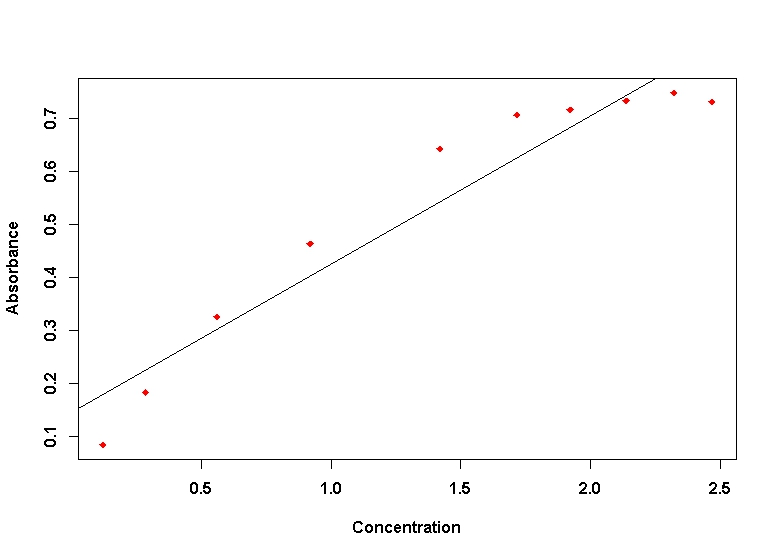
\includegraphics[scale=0.55]{ExamQ3plot}
\end{center}


\begin{itemize}
\item[i.] (1 marks) Is the simple linear regression model approach suitable for this study? Explain your answer with reference to the scatter-plot.
\item[ii] (3 marks) Two polynomial models were  fitted to the data. Description of all three fitted models are found in the three blocks of \texttt{R} code below. The \emph{Akaike information criterion} is listed, for each of the three fitted models. Write down the regression equations fo each ofthe three models.

\item[iv.] (2 marks) Specify which one of the models you would use. Justify your answer with appropriate statistical values.
\end{itemize}


%
%
%
%\item[(d)] Two polynomial models were also fitted to the data. Description of all three fitted models are found in the three blocks of \texttt{R} code below. The \emph{Akaike information criterion} is also listed, for each of the three fitted models.
%\begin{itemize}
%\item[i.] (4 marks) Write down the regression equation for each of the three linear models.
%\item[ii.] (2 marks) Based on the \emph{Akaike information criterion}, which fitted model can be assumed to be the best fit of the three candidate models.
%\item[iii.] (2 marks) Using the best fit model, predict a value for absorbance when the concentration level is 1.2 $mg/ml$.
%\end{itemize}
%\newpage
\begin{itemize}
\begin{framed}
\item[\textbf{Model 1}]
\begin{verbatim}
> summary(Model1)
Call:
lm(formula = Absorb ~ Conc)
...
Coefficients:
              Estimate Std. Error t value Pr(>|t|)
(Intercept)    0.14412    0.04721   3.053   0.0158 *
Concentration  0.28088    0.02930   9.586 1.16e-05 ***
---
Signif. codes:  0 �***� 0.001 �**� 0.01 �*� 0.05 �.� 0.1 � � 1

Residual standard error: 0.07584 on 8 degrees of freedom
Multiple R-squared: 0.9199,     Adjusted R-squared: 0.9099
F-statistic: 91.89 on 1 and 8 DF,  p-value: 1.163e-05
>
>AIC(Model1)
[1] -19.4343
\end{verbatim}
\end{framed}

\begin{framed}
\item[\textbf{Model 2}]
\begin{verbatim}
> summary(Model2)
Call:
lm(formula = Absorb ~ Conc + Conc.Squared)
...
Coefficients:
               Estimate Std. Error t value Pr(>|t|)
(Intercept)    0.006582   0.008013   0.821    0.439
Concentration  0.642935   0.015568  41.299 1.27e-09 ***
Conc.Squared  -0.140573   0.005894 -23.851 5.79e-08 ***
---
Signif. codes:  0 �***� 0.001 �**� 0.01 �*� 0.05 �.� 0.1 � � 1

Residual standard error: 0.008939 on 7 degrees of freedom
Multiple R-squared: 0.999,      Adjusted R-squared: 0.9987
F-statistic:  3592 on 2 and 7 DF,  p-value: 2.879e-11
>
> AIC(Model2)
[1] -61.5338
\end{verbatim}
\end{framed}

\newpage
\begin{framed}
\item[\textbf{Model 3}]
\begin{verbatim}
> summary(Model3)

Call:
lm(formula = Absorb ~ Conc+ Conc.Squared + Conc.Cubed)
...
...
Coefficients:
               Estimate Std. Error t value Pr(>|t|)
(Intercept)    0.013712   0.011629   1.179   0.2830
Concentration  0.608682   0.042825  14.213 7.58e-06 ***
Conc.Squared  -0.108186   0.038088  -2.840   0.0296 *
Conc.Cubed    -0.008196   0.009518  -0.861   0.4223
---
Signif. codes:  0 �***� 0.001 �**� 0.01 �*� 0.05 �.� 0.1 � � 1

Residual standard error: 0.009109 on 6 degrees of freedom
Multiple R-squared: 0.9991,     Adjusted R-squared: 0.9987
F-statistic:  2306 on 3 and 6 DF,  p-value: 1.422e-09
>
> AIC(Model3)
[1] -60.69903
\end{verbatim}
\end{framed}
\end{itemize}
%
\end{itemize}% End of Question
%
%%\end{document}
%--------------------------------------------------------%
\newpage
\subsection*{Question 3. (20 marks) Statistical Process Control }




\begin{itemize}
\item[(a)] Answer the following questions.

\begin{itemize}
\item[i.] (1 marks) What is the purpose of maintaining control charts?
\item[ii.] (1 marks) What is the \emph{Three Sigma} rule in the context of statistical process control?
\item[iii.] (4 marks) Other than applying the \emph{Three Sigma} rule for detecting the presence of an assignable cause, what else do we look for when studying a control chart? Limit your answer to three examples. Support your answer with sketches.
\item[iv.] (2 Marks) What is a CUSUM chart? What type of departures from the production target value
is this type of chart useful for detecting?
\end{itemize}

\item[(b)] A normally distributed quality characteristic is monitored through the use of control charts. These charts have the following parameters. All charts are in control.
\begin{center}
\begin{tabular}{|c|c|c|c|}
\hline  & LCL & Centre Line & UCL \\
\hline $\bar{X}$-Chart & 614 & 620 & 626 \\
\hline $R$-Chart & 0 & 8.236 & 18.795 \\ \hline
\end{tabular}
\end{center}

\begin{itemize}
\item[i.] (2 marks) What sample size is being used for this analysis?
\item[ii.] (2 marks) Estimate the standard deviation of this process.
\item[iii.] (2 marks) Compute the control limits for the process standard deviation chart (i.e. the s-chart).
\end{itemize}

\item[(c)] An automobile assembly plant concerned about quality improvement measured sets of five camshafts on twenty occasions throughout the day. The specifications for the process state that the design specification limits at 600$\pm$3mm.


\begin{itemize}
\item[i.] (2 marks) Determine the \emph{Process Capability Indices} $C_p$ and $C_{pk}$, commenting on the respective values. You may use the \texttt{R} code output on the following page.
\item[ii.] (2 marks)  The value of $C_{pm}$ is $1.353$. Explain why there would be a discrepancy between $C_p$ and $C_{pm}$.
\item[iii.] (2 marks) Comment on the graphical output of the \emph{Process Capability Analysis}, also presented on the next page.
\end{itemize}


\newpage
\begin{framed}
\begin{verbatim}
Process Capability Analysis

Call:
process.capability(object = obj, spec.limits = c(597, 603))
Number of obs = 100          Target = 600
       Center = 599.548         LSL = 597
       StdDev = 0.5846948       USL = 603

Capability indices:
      Value   2.5%  97.5%
Cp    ...
Cp_l  ...
Cp_u  ...
Cp_k  ...
Cpm   1.353  1.134  1.572
Exp<LSL 0%   Obs<LSL 0%
\end{verbatim}
\end{framed}



\begin{center}
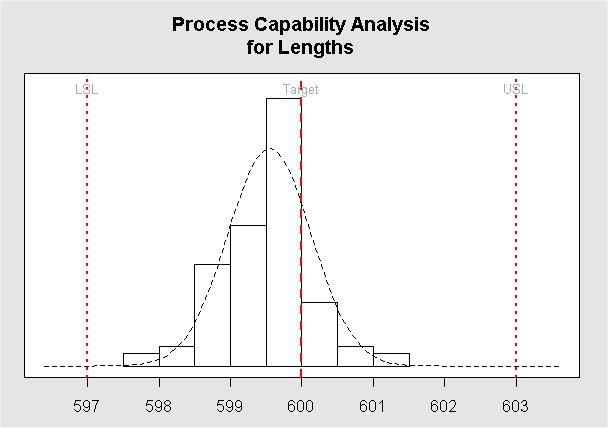
\includegraphics[scale=0.55]{ExamQ4hist}
\end{center}
\newpage
%
%Lengths = Values
%
%obj <- qcc(Lengths, type="xbar")
%
%process.capability(obj, spec.limits=c(597,603))
\end{itemize}


%-----------------------------------------------------------%
\newpage

\subsection*{Question 4. (20 marks) Experimental Design Part 1}

% Definitions
% One Way ANOVA
% Checking Assumptions

\begin{itemize}
\item[(a)] Explain the following terms in the context of experimental design
\begin{itemize}
\item[i.] (2 marks) levels of a factor.
\item[ii.] (2 marks) randomized block design.
\end{itemize}


\item[(b)] Six analysts each made seven determinations of the paracetamol content of the same batch of tablets.
The results are shown below. There are 42 determinations in total. The mean determination for each analysts is also tabulated. \\


%Analyst= structure(c(1L, 2L, 3L, 4L, 5L, 6L, 1L, 2L, 3L, 4L, 5L, 6L, 1L,
%2L, 3L, 4L, 5L, 6L, 1L, 2L, 3L, 4L, 5L, 6L, 1L, 2L, 3L, 4L, 5L,
%6L, 1L, 2L, 3L, 4L, 5L, 6L, 1L, 2L, 3L, 4L, 5L, 6L), .Label = c("A",
%"B", "C", "D", "E", "F"), class = "factor")

%Determinations= c(84.32, 84.24, 84.29, 84.14, 84.5, 84.7, 84.61, 84.13, 84.28,
%84.48, 83.91, 84.36, 84.64, 84, 84.4, 84.27, 84.11, 84.61, 84.62,
%84.02, 84.63, 84.22, 83.99, 84.15, 84.51, 84.25, 84.4, 84.22,
%83.88, 84.17, 84.63, 84.41, 84.68, 84.02, 84.49, 84.11, 84.51,
%84.3, 84.36, 84.33, 84.06, 83.81)

\begin{center}
\begin{tabular}{|c|ccccccc|}
\hline
Analyst	& Content		&		&		&		&		&		&		 \\ \hline
A	&	84.32	&	84.61	&	84.64	&	84.62	&	84.51	&	84.63	&	84.51	 \\
B	&	84.24	&	84.13	&	84.00	&	84.02	&	84.25	&	84.41	&	84.30	 \\
C	&	84.29	&	84.28	&	84.40	&	84.63	&	84.40	&	84.68	&	84.36	 \\
D	&	84.14	&	84.48	&	84.27	&	84.22	&	84.22	&	84.02	&	84.33	 \\
E	&	84.50	&	83.91	&	84.11	&	83.99	&	83.88	&	84.49	&	84.06	 \\
F	&	84.70	&	84.36	&	84.61	&	84.15	&	84.17	&	84.11	&	83.81	 \\
\hline
\end{tabular}
\end{center}
\bigskip
The following \texttt{R} output has been produced as a result of analysis of these data:

%Experiment=data.frame(Determinations, Analyst)
%Model=aov(Determinations~Analyst)
%summary(Model)

%Analysis of Variance Table
%
%            Df Sum Sq Mean Sq F value  Pr(>F)
%Analyst      5 0.8611 0.17222   4.236 0.00394 **
%Residuals   36 1.4635 0.04065
%---
%Signif. codes:  0 �***� 0.001 �**� 0.01 �*� 0.05 �.� 0.1 � � 1

\begin{center}
\texttt{
\begin{tabular}{|c|cccccc|}
  \hline
  % after \\: \hline or \cline{col1-col2} \cline{col3-col4} ...
	&&		&		&		&		&		\\
  Response: Y        	&&	Df  	&	Sum Sq 	&	Mean Sq 	&	F value    	&	$Pr(>F)$    	\\
  	&&		&		&		&		&		\\\hline
	&&		&		&		&		&		\\
Analyst 	&&	\textbf{?}	&	\textbf{?}	&	\textbf{?}	&	\textbf{?}	&	0.00394 **	\\
	&&		&		&		&		&		\\ \hline
&&		&		&		&		&		\\
Residuals	&&	\textbf{?}	&	\textbf{?}	&	0.04065	&	&		\\
	&&		&		&		&		&		\\ \hline
&&		&		&		&		&		\\
Total	&&	\textbf{?}	&	2.3246	&		&		&		\\
	&&		&		&		&		&		\\ \hline
\end{tabular}
}
\end{center}
\begin{itemize}
\item[i.] (5 marks) Complete the ANOVA table in your answer sheet, replacing the "?" entries with the correct values.
\item[ii.] (2 marks) What hypothesis is being considered by this procedure.
\item[iii.] (2 marks) What is the conclusion following from the above analysis? State the null and alternative hypothesis clearly.
\end{itemize}
\newpage

\item[(c)] The \texttt{R} code and graphical procedures, below and on the following page, are relevant to checking whether the underlying assumptions are met for the ANOVA model in part (b).
\begin{itemize}
\item[i.] (3 marks) What are the assumptions underlying ANOVA?
\item[ii.] (4 marks)  Assess the validity of these assumptions for the ANOVA model in part(b).

\end{itemize}
\begin{framed}
\begin{verbatim}
        Shapiro-Wilk normality test

data:  Residuals
W = 0.9719, p-value = 0.3819
\end{verbatim}
\end{framed}
\begin{framed}
\begin{verbatim}
        Bartlett test of homogeneity of variances

data:  Experiment
Bartlett's K-squared = 105.9585, df = 1, p-value < 2.2e-16
\end{verbatim}
\end{framed}
\begin{center}
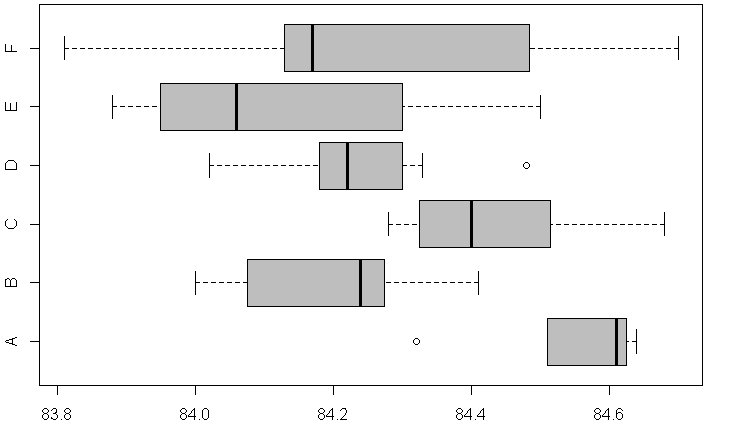
\includegraphics[scale=0.59]{ExamQ5boxplot}
\end{center}
\newpage
%qqnorm(resid(Model),pch=18,col="red",font.lab=2,font.axis=2)
%qqline(resid(Model))
\begin{center}
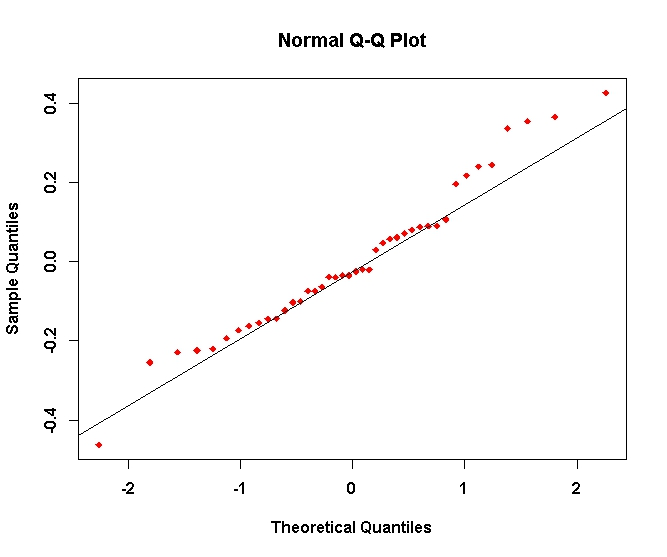
\includegraphics[scale=0.55]{ExamQ5qqplot}
\end{center}
\begin{center}
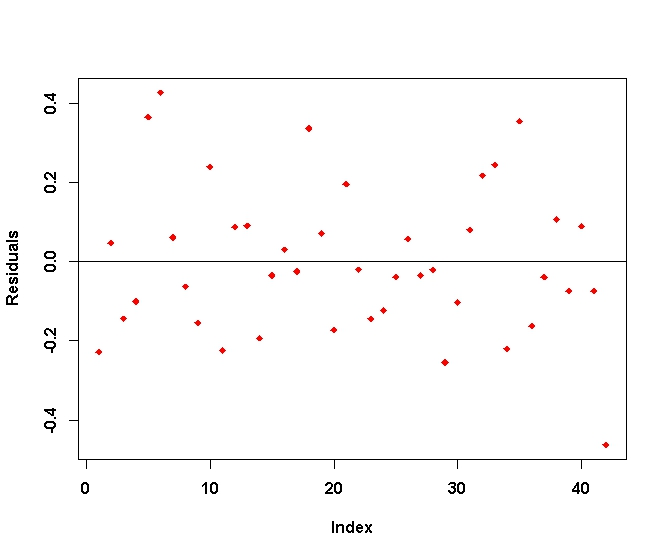
\includegraphics[scale=0.55]{ExamQ5resid}
\end{center}
\end{itemize}

%-----------------------------------------------------------------%
%-----------------------------------------------------------------%
\newpage
\subsection*{Question 5. (20 marks) Experimental Design Part 2 }
\begin{itemize} % Start of Question 5
\item[(a)] % Part A

In an investigation into the extraction of nitrate-nitrogen from air dried soil, three quantitative variables were investigated at two levels. These were the amount of oxidised activated charcoal (A) added to the extracting solution to remove organic interferences, the strength of CaSO4 extracting solution (C), and the time the soil was shaken with the solution (T). The aim of the investigation was to optimise the extraction procedure. The levels of the variables are given here:
\begin{center}
{
\large
\begin{tabular}{|cc|c|c|}
\hline	&		&\phantom{sp}	{\LARGE -}\phantom{sp}	&	\phantom{sp} {\LARGE +} \phantom{sp}	\\ \hline
Activated charcoal (g) 	&	A 	&	0.5	&	1	\\ \hline
CaSO{4} (\%) 	&	C 	&	0.1	&	0.2	\\ \hline
Time (minutes) 	&	T 	&	30	&	60	\\ \hline
\end{tabular} 
}
\end{center}

The concentrations of nitrate-nitrogen were determined by ultra-violet spectrophotometry and compared with concentrations determined by a standard technique. The results are given below and are the amounts recovered (expressed as the percentage of known nitrate concentration).
{
\large
\begin{center}
\begin{tabular}{|c|c|c|cc|}
  \hline
\phantom{sp}A\phantom{sp}	&	\phantom{sp}C\phantom{sp}	&\phantom{sp}	T\phantom{sp}	&	Amounts&	(2 Replicates)	\\
  \hline
-1	&	-1	&	-1	&	45.1	&	44.6	\\ \hline
									
1	&	-1	&	-1	&	44.9	&	45.3	\\ \hline
									
-1	&	1	&	-1	&	44.8	&	46.7	\\ \hline
									
1	&	1	&	-1	&	44.7	&	44.8	\\ \hline
									
-1	&	-1	&	1	&	33	&	35	\\ \hline
									
1	&	-1	&	1	&	53.8	&	51.7	\\ \hline
									
-1	&	1	&	1	&	32.6	&	33.7	\\ \hline							
1	&	1	&	1	&	54.2	&	53.2	\\ \hline
\end{tabular}
\end{center}
}
\end{itemize}


\newpage


\begin{itemize}
\item[i.] (8 Marks) Calculate the contrasts, the effects and the sum of squares for the effects.
\item[ii.] (8 Marks) Using the computed sums of squares values, complete the ANOVA table (see the \texttt{R} code below).
\item[iii.] (4 Marks) Comment on the tests for significant for the main effects and interactions. State clearly your conclusions.
\item[iv.] (4 Marks) Write down a  regression equation that can be used predicting amounts based on the results of this experiment.
\end{itemize}

\begin{framed}
\begin{verbatim}
            Df Sum Sq Mean Sq F value     Pr(>F)    
A            1    ...     ...     ...   0.000979 ***
C            1    ...     ...     ...   0.934131    
T            1    ...     ...     ...   0.395554 
A:C          1    ...     ...     ...   0.944243    
A:T          1    ...     ...     ...   0.017582 *
C:T          1    ...     ...     ...   0.072101
A:C:T        1    ...     ...     ...   0.028522 *    
Residuals    8  116.2    14.5                      
\end{verbatim}
\end{framed}

\newpage
\begin{center}
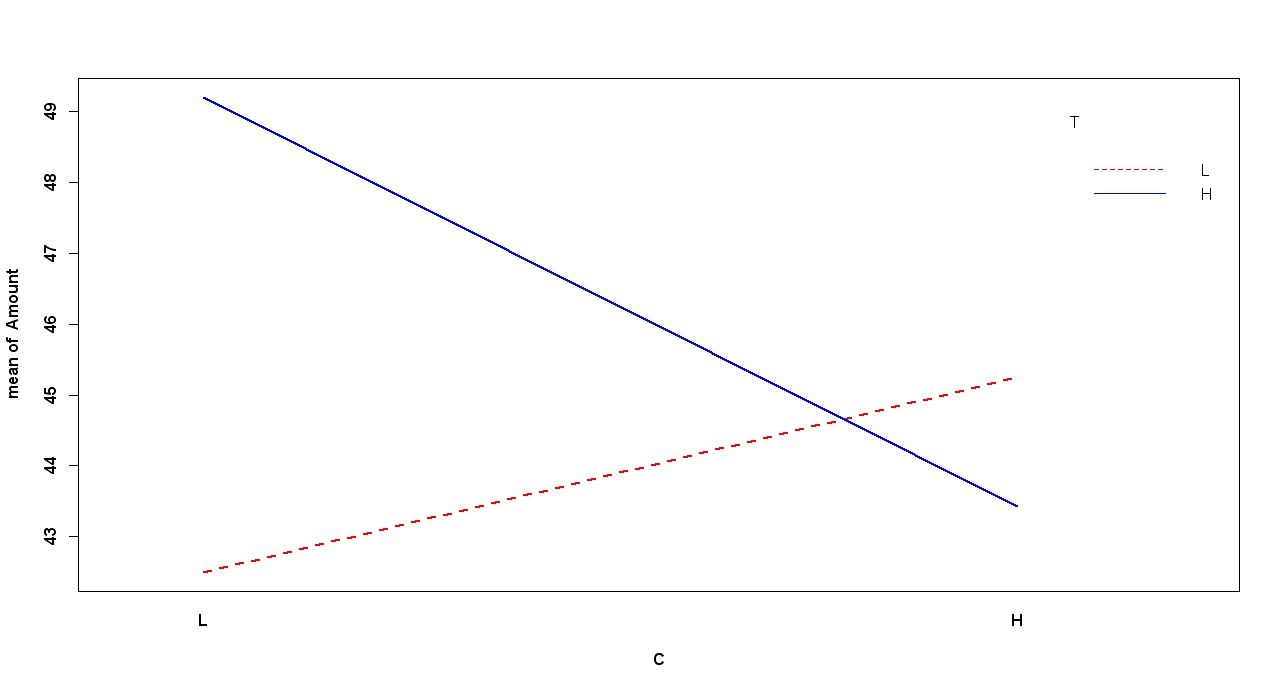
\includegraphics[scale=0.3]{ExamQ6interactionanew}
\end{center}
\begin{center}
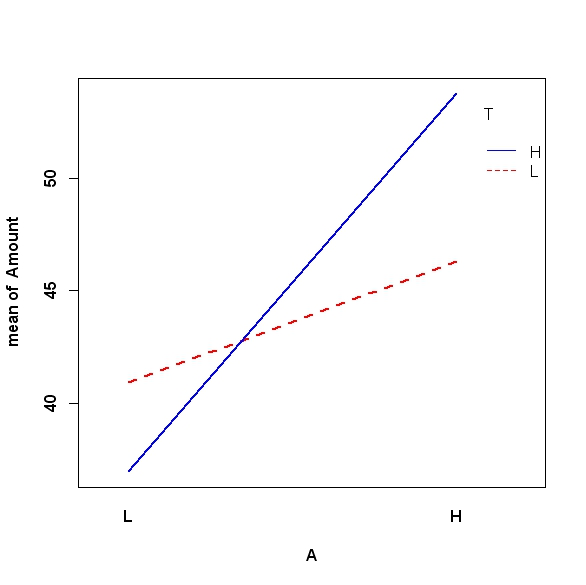
\includegraphics[scale=0.3]{ExamQ6interactionbnew}
\end{center}
\begin{center}
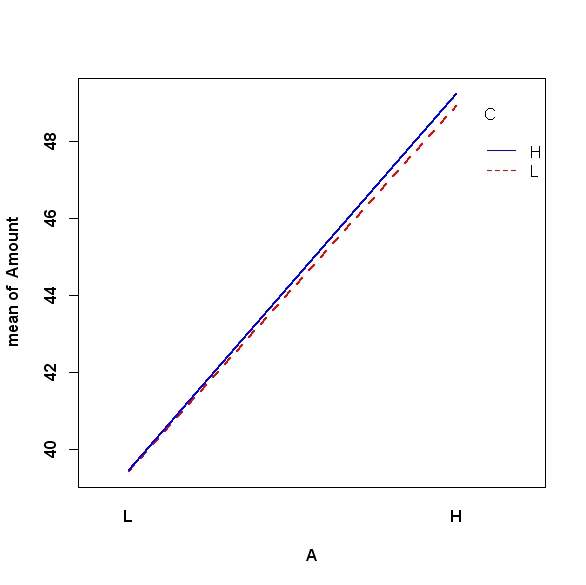
\includegraphics[scale=0.3]{ExamQ6interactioncnew}
\end{center}

 % End of Question
\newpage
\large{
\subsection*{Control Limits for Control Charts}

 \[ \bar{\bar{x}} \pm 3\frac{\bar{s}}{c_4\sqrt{n}}\]

 \[ \bar{s} \pm 3\frac{c_5\bar{s}}{c_4}\]

 \[\left[ \bar{R}D_3, \bar{R}D_4\right]\]

\subsection*{Process Capability Indices}
\[ \hat{C}_p = \frac{\mbox{USL} - \mbox{LSL}}{6s}\]

\[ \hat{C}_{pk} = \mbox{min} \left[\frac{\mbox{USL} - \bar{x}}{3s},\frac{\bar{x} - \mbox{LSL}}{3s} \right] \]

\[ \hat{C}_{pm} = \frac{\mbox{USL} - \mbox{LSL}}{6\sqrt{s^2+(\bar{x}-T)^2}}\]
\bigskip
%\subsection*{2^3 Design: Main Effect}
%
%\[X= \frac{1}{4n} \left[ x + xy + xz + xyz - (1) - y - z - yz \right]\]
%\bigskip
\subsection*{$2^3$ Design: Interaction Effects}

\[ AB = \frac{1}{4n} \left[ abc - bc + ab - b - ac + c - a + (1) \right] \]

\[ AC = \frac{1}{4n} \left[ (1) - a + b - ab -c + ac - bc + abc \right] \]

\[ BC = \frac{1}{4n} \left[ (1) + a - b - ab - c - ac + bc + abc \right] \]

\[ABC = \frac{1}{4n} \left[ abc - bc - ac + c - ab + b +  a - (1) \right] \]

\bigskip

\subsection*{Factorial Design: Sums of Squares}

\[\mbox{Effect} =  \frac{\mbox{(Contrast)}}{n2^{k-1}}\]

\[\mbox{Sums of Squares} =  \frac{\mbox{(Contrast)}^2}{n2^k}\]
}
%------------------------------------------------------------------------ %
\Large{
\subsection*{Factors for Control Charts}
\begin{tabular}{|c|c|c|c|c|c|c|}
\hline
Sample Size (n) 	&	c4 	&	c5 	&	d2 	&	d3 	&	D3 	&	D4	\\	\hline
2	&	0.7979	&	0.6028	&	1.128	&	0.853	&	0	&	3.267	\\	
3	&	0.8862	&	0.4633	&	1.693	&	0.888	&	0	&	2.574	\\	
4	&	0.9213	&	0.3889	&	2.059	&	0.88	&	0	&	2.282	\\	
5	&	0.9400	&	0.3412	&	2.326	&	0.864	&	0	&	2.114	\\	
6	&	0.9515	&	0.3076	&	2.534	&	0.848	&	0	&	2.004	\\	
7	&	0.9594	&	0.282	&	2.704	&	0.833	&	0.076	&	1.924	\\	
8	&	0.9650	&	0.2622	&	2.847	&	0.82	&	0.136	&	1.864	\\	
9	&	0.9693	&	0.2459	&	2.970	&	0.808	&	0.184	&	1.816	\\	
10	&	0.9727	&	0.2321	&	3.078	&	0.797	&	0.223	&	1.777	\\	
11	&	0.9754	&	0.2204	&	3.173	&	0.787	&	0.256	&	1.744	\\	
12	&	0.9776	&	0.2105	&	3.258	&	0.778	&	0.283	&	1.717	\\	
13	&	0.9794	&	0.2019	&	3.336	&	0.770	&	0.307	&	1.693	\\	
14	&	0.9810	&	0.1940	&	3.407	&	0.763	&	0.328	&	1.672	\\	
15	&	0.9823	&	0.1873	&	3.472	&	0.756	&	0.347	&	1.653	\\	
16	&	0.9835	&	0.1809	&	3.532	&	0.750	&	0.363	&	1.637	\\
17	&	0.9845	&	0.1754	&	3.588	&	0.744	&	0.378	&	1.622	\\
18	&	0.9854	&	0.1703	&	3.64	&	0.739	&	0.391	&	1.608	\\
19	&	0.9862	&	0.1656	&	3.689	&	0.734	&	0.403	&	1.597	\\
20	&	0.9869	&	0.1613	&	3.735	&	0.729	&	0.415	&	1.585	\\
21	&	0.9876	&	0.1570	&	3.778	&	0.724	&	0.425	&	1.575	\\
22	&	0.9882	&	0.1532	&	3.819	&	0.720	&	0.434	&	1.566	\\
23	&	0.9887	&	0.1499	&	3.858	&	0.716	&	0.443	&	1.557	\\
24	&	0.9892	&	0.1466	&	3.895	&	0.712	&	0.451	&	1.548	\\
25	&	0.9896	&	0.1438	&	3.931	&	0.708	&	0.459	&	1.541	\\
\hline
\end{tabular}
} % End Large Font
\end{document}




